\documentclass[letterpaper,twocolumn,10pt]{article}


\usepackage{usenix}

% === 你原来的功能性宏包（按依赖顺序稍作整理） ===
\usepackage{float}
\usepackage{amsmath}
\usepackage{xspace}
\usepackage{siunitx}
\usepackage{enumitem}
\usepackage{listings}   % 虽然你主要用 minted，但保留无妨
\usepackage{minted}
\usepackage{tikz}
\usetikzlibrary{shapes,arrows,positioning,fit}
\usepackage{subcaption}
\usepackage{balance}
\usepackage{url}
\usepackage{comment}

% 超链接务必尽量靠后加载
\usepackage{hyperref}

% cleveref 在 hyperref 之后加载更稳妥
\usepackage{cleveref}

% === minted 设置 ===
\newlength{\mintednumbersep}
\AtBeginDocument{%
  \sbox0{\tiny00}%
  \setlength\mintednumbersep{\parindent}%
  \addtolength\mintednumbersep{-\wd0}%
}

\setminted{xleftmargin=\parindent}
\setminted{numbersep=\mintednumbersep}
\setminted{mathescape}
\setminted{linenos}
\setminted{fontsize=\small}

% === 你的命令 ===
\newcommand*\circled[1]{\tikz[baseline=(char.base)]{
  \node[shape=circle,draw=black!80,line width=0.2mm,inner sep=0.1pt] (char) {#1};}}

\newcommand{\sys}{gbpf\xspace}
\newcommand{\tech}{GPU eBPF Extension Framework\xspace}
\newcommand{\speedup}{10\%}

\newcommand{\eg}{e.g.,\xspace}
\newcommand{\ie}{i.e.,\xspace}
\newcommand{\etc}{etc.\xspace}

% Cleveref 格式
\crefname{algocf}{algorithm}{algorithms}
\Crefname{algocf}{Algorithm}{Algorithms}
\crefformat{section}{\S#2#1#3}
\Crefformat{section}{Section~#2#1#3}
\crefformat{subsection}{\S#2#1#3}
\Crefformat{subsection}{Section~#2#1#3}
\crefformat{subsubsection}{\S#2#1#3}
\Crefformat{subsubsection}{Section~#2#1#3}
\crefformat{figure}{figure~#2#1#3}
\Crefformat{figure}{Figure~#2#1#3}

% Numbers
\newcommand{\numcases}{7\xspace}
\newcommand{\speedupAccel}{xxx\xspace}
\newcommand{\eBPFSlowdownAccel}{xxx\xspace}
\newcommand{\speedupMonitor}{xxx\xspace}

%%% 紧凑的枚举环境
\newenvironment{smenumerate}%
  {\begin{enumerate}[itemsep=-0pt, parsep=0pt, topsep=0pt, leftmargin=2pc]}
  {\end{enumerate}}

\newenvironment{smitemize}%
  {\begin{list}{$\bullet$}%
    {\setlength{\parsep}{0pt}%
      \setlength{\topsep}{0pt}%
      \setlength{\leftmargin}{2pc}%
      \setlength{\itemsep}{1pt}}}
  {\end{list}}

% 内部批注（提交版记得全部注释掉）
\newcommand{\grumbler}[3]{\noindent{\color{#1}{\bf \fbox{#2}} {\it #3}}}
\newcommand{\arq}[1]{\grumbler{red}{ARQ}{#1}}
\newcommand{\yy}[1]{\grumbler{blue}{YY}{#1}}
\newcommand{\yusheng}[1]{\grumbler{green}{YS}{#1}}
\newcommand{\xiangyu}[1]{\grumbler{orange}{XG}{#1}}
\newcommand{\todo}[1]{\grumbler{olive}{todo}{#1}}

% === 正文开始 ===
\begin{document}


\pagestyle{plain}

% 不打印日期
\date{}


\title{gBPF: A Unified, Safe, and Efficient Policy Runtime for GPU-Centric Systems}


\author{
}

\maketitle

% === 你原来的结构 ===
\begin{abstract}
Modern GPU-centric systems run heterogeneous workloads such as LLM inference, training, and vector search, whose performance and cost are dominated by policies for memory placement, kernel scheduling, and observability. Today, these policies are hard-coded inside framework-specific runtimes, proprietary vendor libraries, and monolithic kernel and device code, leaving operators unable to adapt them to workload mix, SLAs, or hardware changes without invasive code changes and disruption. Prior work has shown that externalizing CPU-side policies with eBPF---for scheduling, cache management, and congestion control---dramatically improves flexibility, but directly applying this pattern to GPUs is difficult. GPU driver mechanisms are tightly intertwined with low-level hardware interactions and lack safe extension points, and programmability on only the host or only the device cannot express coherent end-to-end policies.

We present \sys, a unified, safe, and efficient programmable policy runtime that spans both the CPU host and GPU devices. \sys refactors the GPU driver to expose stable, eBPF-based hooks at key control points, and offloads verified eBPF programs to execute directly inside GPU kernels via a lightweight, sandboxed PTX JIT, all over a shared map abstraction that provides cross-layer state. This design enables workload-specific policies for memory offloading, kernel admission and preemption, and fine-grained observability to run exactly where decisions occur, while preserving safety and low overhead.

We implement \sys on Linux with an extended \sysdriver and a GPU-side runtime, and evaluate it on realistic workloads including LLM inference, GNN training, vector search, and mixed-priority multi-tenant scenarios. Across these settings, \sys-based policies improve throughput by up to $5{\times}$, reduce tail latency by up to $2{\times}$, and add only a few percent runtime overhead for observability. These results demonstrate that unified CPU--GPU extensibility is a practical and necessary foundation for future GPU-centric systems.
\end{abstract}


\section{Introduction}

GPUs now dominate the compute and capital cost of modern datacenters, powering workloads that range from latency-sensitive LLM inference pipelines to large-scale training, graph analytics, and vector search. Across these workloads, end-to-end performance and efficiency are heavily determined not by raw FLOPs, but by \emph{policies}: how the system places and migrates data across device and host memory, how it admits and schedules kernels in multi-tenant environments, and how it collects observability signals to drive online adaptation. These policies must evolve as models, SLAs, and hardware change. Yet today they are largely frozen inside proprietary vendor stacks and per-framework runtimes, making GPU infrastructure rigid and costly to operate.

In current GPU stacks, the host driver and device firmware implement a fixed, closed set of mechanisms for memory management, context scheduling, and performance event collection. Frameworks such as PyTorch or TensorFlow, and emerging inference runtimes such as vLLM, build bespoke management logic on top of these mechanisms, often by defensively hoarding GPU memory or hard-wiring scheduling heuristics for a specific workload mix. Because the underlying mechanisms expose no safe extension points, operators cannot express workload-specific policies for memory placement or preemption at the points where they matter --- for example, when a kernel require a memory offloaded to CPU or when a low-priority job is about to delay a latency-critical query. As a result, datacenter GPU deployments suffer from unpredictable tail latency, underutilization, and frequent disruption when policies must be revised or tuned.

By contrast, the CPU side of modern systems has undergone a steady shift toward programmable policies. The extended Berkeley Packet Filter (eBPF) ecosystem now supports dynamically loaded, verified programs for scheduling (\texttt{sched\_ext}), page-cache eviction (\texttt{cache\_ext}), TCP congestion control (\texttt{struct\_ops}), and a wide body of observability tools~\cite{gregg16,gregg2021computing,Bachl21,Zhong22,jia2023programmable,bpftime}. In these designs, a small set of stable kernel mechanisms is exposed through structured attach points, and BPF programs implement policies that can be updated at runtime without rebooting or patching the kernel~\cite{schedext-docs,cacheext-docs}. It is tempting to apply the same idea to GPUs: treat the GPU driver as another kernel subsystem, attach host-side BPF programs to its control paths, and use those to implement adaptive GPU policies.

However, directly extending host-only BPF to GPU-centric systems fails for two fundamental reasons. First, many critical decisions --- such as whether to prefetch or evict certain data, how to throttle or prioritize individual warps, or when a kernel is triggering pathological memory behavior --- are made on the device, within GPU kernels and on-chip schedulers that are invisible to host-only instrumentation. Second, monolithic GPU drivers tightly couple resource management with low-level hardware protocols (e.g., MMU updates, interrupt handling, context teardown) and provide no stable, documented hooks; naively inserting probes risks GPU hangs, kernel panics, or subtle resource leaks. Conversely, GPU-only instrumentation tools such as CUPTI, NVBit, Neutrino, and eGPU~\cite{cupti,villa2019nvbit,neutrino,eGPU} provide rich telemetry by rewriting PTX or SASS, and recent userspace eBPF runtimes such as bpftime can inject BPF-like code into GPU kernels~\cite{bpftime}, but they are designed for profiling rather than online policy enforcement, lack a unified safety model with the OS, and do not integrate with privileged driver mechanisms.

Designing a general substrate for GPU policy programmability therefore raises several challenges. \emph{C1: Safe driver extensibility.} We must retrofit mechanism–policy separation into large, performance-critical GPU drivers without destabilizing their low-level interaction with hardware. \emph{C2: Safe and efficient device-side execution.} We need to execute user-supplied policy logic inside GPU kernels, on the critical path of memory accesses and synchronization, while guaranteeing bounded execution and memory safety in a massively parallel environment. \emph{C3: cross-layer state and metadata.} Policies often need to correlate host-side and device-side signals (e.g., page access patterns with warp-level stalls); doing so requires a shared state abstraction and efficient synchronization across the CPU–GPU boundary. \emph{C4: A single safety and control plane.} Finally, the policy runtime must support unified verification, deployment, and debugging for both host and device execution contexts; otherwise, operators are left with another fragmented stack of heterogeneous mechanisms.

We present \sys, a unified, safe, and efficient policy runtime for GPU-centric systems that addresses these challenges. \sys exposes a small set of stable, low-level GPU mechanisms---for memory placement and migration, kernel admission and preemption, and kernel-level instrumentation---as programmable attach points in an extended GPU driver. Policies are expressed as eBPF programs in a restricted instruction subset and are statically verified for memory safety and bounded execution. The same eBPF intermediate representation is then offloaded to GPU devices: \sys translates verified bytecode into PTX, injects it at kernel launch time via lightweight trampolines, and executes it inside kernels within a sandboxed runtime. Both host- and device-side policy code share a common map abstraction backed by unified memory, providing low-latency cross-layer state without manual data marshalling.

We implement \sys on Linux by extending \sysdriver over NVIDIA's open GPU kernel modules and by building a GPU-side PTX JIT and sandbox runtime. The driver modifications follow a \texttt{struct\_ops}-style pattern: they introduce a handful of attach points in memory-management and scheduling paths without restructuring existing mechanisms, and delegate decisions to verified eBPF callbacks. On the device side, lightweight PTX trampolines save minimal register state, invoke the translated eBPF snippet, and restore state to resume execution, adding sub-microsecond overhead in our microbenchmarks. Unlike prior GPU observability tools~\cite{cupti,villa2019nvbit,neutrino,eGPU} or userspace BPF runtimes~\cite{bpftime}, \sys offers one cross-layer policy model spanning the driver and the device, under a single verifier and control plane.

We evaluate \sys on realistic GPU datacenter workloads including LLM inference pipelines, graph neural network training, vector search, and mixed-priority multi-tenant scenarios. Using \sys, we implement adaptive memory placement and eviction, fine-grained kernel admission and preemption, and bcc-style observability tools for GPU kernels. Across these workloads, \sys-based policies improve throughput by up to $5{\times}$ and cut p99 latency by up to $2{\times}$ compared to static heuristics, while instrumentation-only deployments incur $2$–$3\%$ overhead. These results suggest that exposing unified, eBPF-style policy programmability across CPU and GPU is a practical and powerful abstraction for managing GPU-centric systems.

\begin{itemize}[leftmargin=*,itemsep=0pt]
    \item We identify and characterize key programmability gaps in GPU stacks for memory management, scheduling, and observability, and show how they lead to brittle, hard-coded policies that cannot adapt to evolving workloads.
    \item We introduce \sys, the first system to provide a unified eBPF-based policy runtime that spans CPU and GPU execution contexts, combining verified driver hooks with safe, JIT-compiled execution of BPF programs inside GPU kernels over a shared state abstraction.
    \item We demonstrate that \sys enables adaptive, workload-specific policies that significantly improve performance, utilization, and tail latency for realistic LLM inference, training, and vector workloads, with low overhead and without application or driver rewrites.
\end{itemize}

\section{Background and Motivation}
\label{sec:background}
\subsection{GPU Systems and Workload Diversity}
\label{sec:arch-gpu}

% \arq{I think this is too many ideas for one paragraph  It should probably reference Figure 1 (!)}
As shown in \Cref{fig:motivation_silos}, we focus on three GPU resource management domains across the software stack: memory placement and migration, compute scheduling, and on-device thread scheduling. User-space frameworks (e.g., vLLM~\cite{kwon2023efficient}, Salus~\cite{yu2020fine}, PILOT~\cite{ravi2021pilot}) leverage application semantics (e.g., neural structures, latency constraints) to implement request scheduling and KV-cache offloading policies. Kernel drivers manage memory, scheduling, and multi-tenant isolation via privileged hardware mechanisms (MMU, interrupts), typically using fixed, application-agnostic algorithms (e.g., LRU eviction) under Unified Virtual Memory (UVM), which transparently handles oversubscription through host-device page migrations. GPU devices execute kernels via SIMT (Single Instruction, Multiple Threads); on NVIDIA hardware, 32-thread warps run instructions in lockstep on SMs, with internal states (e.g., warp access patterns) opaque to host drivers.


\begin{figure}[t]
    \centering
    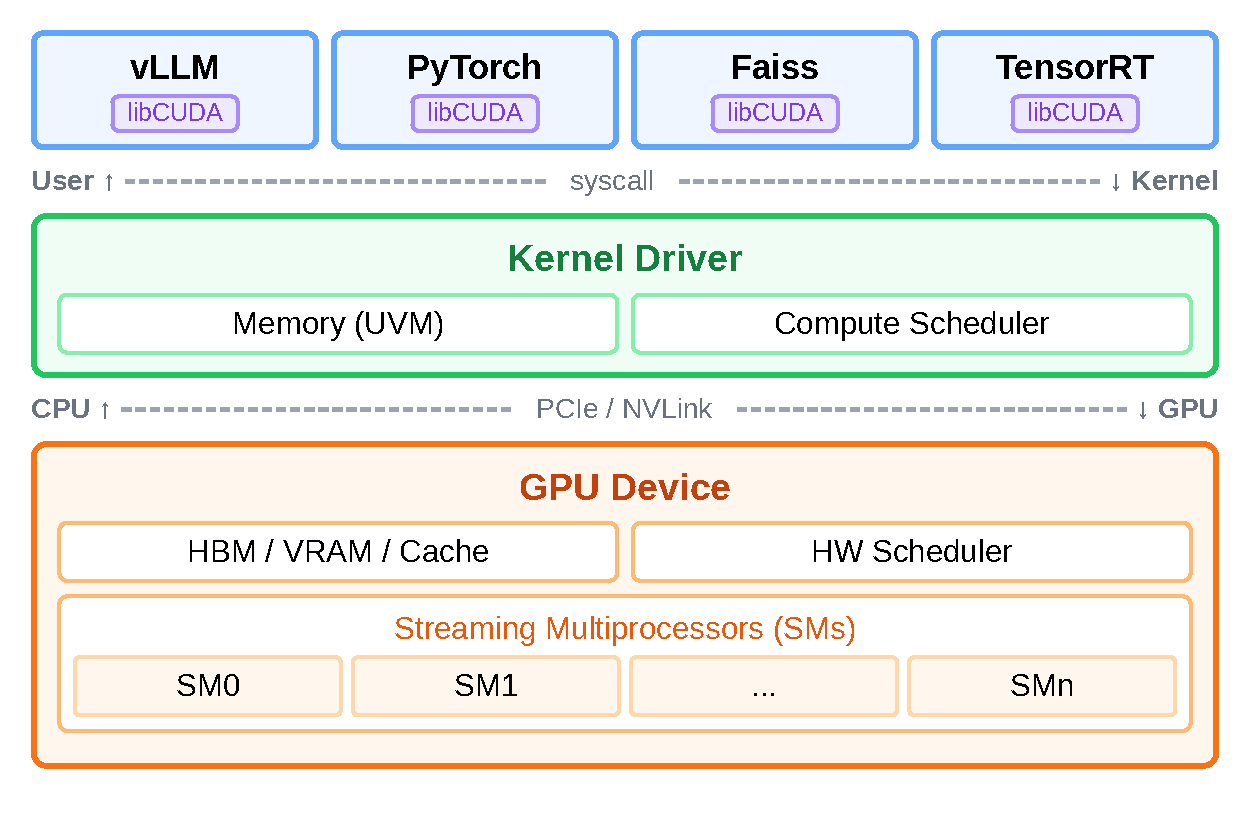
\includegraphics[width=\columnwidth]{img/gpu_stack_figure.pdf}
    \caption{GPU system stack: user-space frameworks, kernel driver (memory and scheduling), and GPU hardware.}
    \label{fig:motivation_silos}
\end{figure}

% \arq{I think this should be two paragraphs: one that talks about workload diversity and the second that then talks about the need for different policies.}
GPU workloads exhibit diverse resource access patterns. Results from \sys{}'s eBPF-based tracing tools (\S\ref{sec:eval}) confirm this diversity: \Cref{fig:access_patterns} captures memory page-fault addresses over time under UVM, showing that LLM MoE inference exhibits periodic stride bursts from expert activations; GNN training shows irregular random access from pointer-chasing graph traversal; and vector search alternates between sequential scans (index build) and random probes (query)~\cite{pan2024survey,cao2023gpu}. \Cref{fig:thread_scheduling} reveals a 127$\times$ SM scheduling load imbalance in a vector-add GPU kernel, invisible to host-side drivers.

These diverse patterns require workload-specific policies across all three domains. UVM eviction and prefetch policies alone can impact execution time by up to 73\%~\cite{ganguly2019interplay,park2025helm}: MoE inference favors specialized eviction over default LRU~\cite{sheng2023flexgen,kwon2023efficient}, while GNN training demands aggressive sequential prefetch~\cite{lin2024towards,wang2016gunrock}, but each can degrade other workloads. Compute scheduling requires adaptive priority and preemption policies as multi-tenant demands fluctuate~\cite{fan2025gpreempt,wang2024gcaps}, and SM load imbalance benefits from custom thread scheduling. Yet current drivers and firmware enforce a single fixed policy.
\begin{figure*}[t]
    \centering
    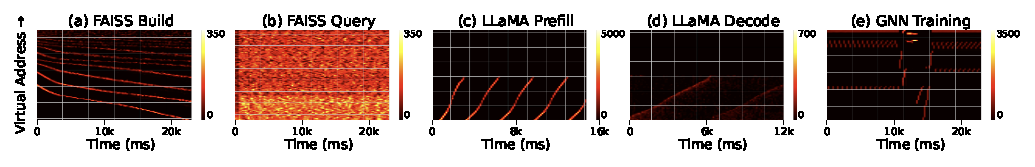
\includegraphics[width=\textwidth]{img/pattern/combined_patterns_1x5_v2.pdf}
    \caption{Page-fault address traces over time across four workloads. Each pattern implies a different optimal prefetch/eviction strategy; no single policy fits all.}
    \label{fig:access_patterns}
\end{figure*}


\begin{figure}[t]
    \centering
    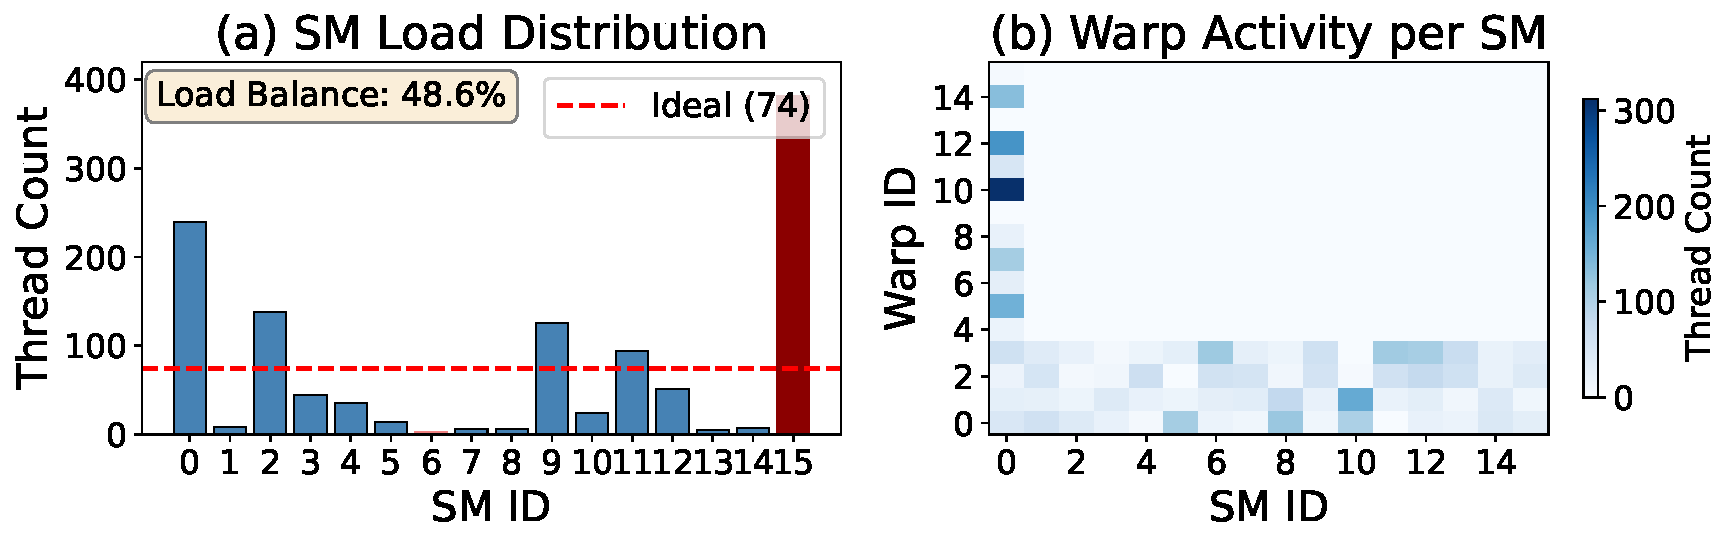
\includegraphics[width=\columnwidth]{img/pattern/vector_add/thread_scheduling_motivation.pdf}
    \caption{GPU thread scheduling imbalance observed via eBPF tracing. (a) SM load distribution: 127$\times$ imbalance. (b) Warp activity heatmap across SMs.}
    \label{fig:thread_scheduling}
\end{figure}

\subsection{Agent-Based Policy Exploration}
\label{sec:motivation-agent}

Agentic OS policy exploration fits the large GPU policy space but requires programmable interfaces at the relevant control boundaries. Unlike parameter-tuning methods, AI agents~\cite{dwivedula2025policysmith,zheng2025schedcp} directly generate and iteratively refine policy logic to explore richer, workload-specific strategies. Ordinary driver/UVM interfaces expose preset controls (e.g., \texttt{cudaMemAdvise}, driver module parameters), rather than arbitrary workload-aware eviction or fault-path prefetch callbacks. Framework and driver extensions can add programmability, with the boundaries discussed below.

Effective GPU policy optimization requires an OS interface with three key properties: (1) \emph{safe}, robustly handling generated policies without kernel panics or GPU corruption; (2) \emph{dynamic}, rapidly deploying and iterating policies at runtime without application restarts or kernel rebuilds; and (3) \emph{full-stack}, observing GPU-internal states, coordinating across tenants, and controlling driver-level decisions like eviction and fault-path prefetching.

\subsection{Limitations of Existing Approaches}
\label{sec:motivation-limitations}

% \arq{Make sure to critique these existing approaches by saying they are not safe, dynamic, or full-stack.}
Existing approaches fail to simultaneously provide a safe, dynamic, and full-stack programmable OS interface for GPU resource management.

\paragraph{Driver-Level Policies}
Driver-level approaches expose preset controls (e.g., \texttt{cudaMemAdvise} and driver module parameters) or add custom control paths. Systems like TimeGraph~\cite{kato2011timegraph}, Gdev~\cite{kato2012gdev}, and OS kernel interception methods~\cite{kernelintercept} embed scheduling or memory-management logic into driver modules. More recent work such as GPREEMPT~\cite{fan2025gpreempt} and GCAPS~\cite{wang2024gcaps} adds priority-based preemption, while LithOS~\cite{coppock2025lithos} provides a redesigned runtime. These systems have different trust and deployment boundaries; a modified driver is not inherently an unsafe implementation. The relevant distinction is whether a policy can change independently of trusted driver code, and which observations and actions its interface exposes. \Cref{tab:policy-expressibility} identifies those boundaries for the policies considered here.

\paragraph{Host User-Space Runtimes and Libraries}
User-space frameworks~\cite{ng2023paella,gim2025pie,shen2025xsched,chen2025ktransformers,coppock2025lithos} can implement rich policies when applications expose the necessary state and controls. Framework integration supplies useful semantics but can require per-framework adapters. A shared user-space scheduler can coordinate participating tenants~\cite{xiao2018gandiva,yu2020fine}; process boundaries do not make such coordination impossible. Ordinary application APIs do not, however, place arbitrary policy code inside a UVM fault handler or expose PMM eviction-list transitions. Device-side instrumentation and cooperating kernels provide other observations and controls, with their own integration requirements. Our comparison therefore concerns specific missing control boundaries, not a blanket inability of user space to schedule across tenants or observe GPU execution.

% Design Principles commented out — too generic, covered by intro and motivation

\section{\sys Design}

% Challenges C1/C2/C3 moved to §3 Motivation (sec:motivation-limitations)

\sys{} is designed to provide a safe, programmable, and workload-adaptive GPU resource management OS interface capable of supporting dynamic, AI-generated policies, transparent to applications. As identified in \S\ref{sec:motivation-limitations}, achieving these goals requires addressing three GPU-specific challenges unmet by existing CPU eBPF models: (1) cross-device latency that necessitates asynchronous policy execution, (2) tight coupling of memory and scheduling decisions demanding unified hooks across these domains, and (3) GPU device opacity requiring device-side verified BPF execution. The following subsections detail how \sys{} addresses these challenges.

\subsection{\sys{} Policy Execution Model}
\label{sec:design-interfaces}

\subsubsection{Programmable Lifecycle and Decoupled Execution}


\sys models GPU resource management as programmable lifecycles. GPU resources transition through defined lifecycles: memory chunks between activated, accessed, and evicted; compute contexts between created, scheduled, preempted and finished. 


To write a policy in \sys{}, Developers implement eBPF programs that attach to events in the lifecycle and direct state transitions using kernel functions (\emph{kfuncs}). In prior BPF extensibility systems, the primary effect is the \emph{return value}: the kernel asks a question at a transition point and the BPF program returns an answer (which CPU to dispatch to, whether to drop a packet). Triggers such as GPU faults, application-level API calls (uprobes), device-side execution events, and async tasks (bpf_wq) can each initiate multiple state transitions asynchronously, thereby decoupling policy triggers from their cross-device effects. This shift is forced by three properties of GPU policy: a single hook must produce multiple concurrent effects (e.g., prefetch and preempt simultaneously), effects must be asynchronous (DMA outlives the callback), and hooks span fundamentally different execution environments (host CPU, user process, GPU SIMT) where no unified return-value format is possible. 
This decoupling is not a design choice but a necessity forced by the cross-device boundary. Prior eBPF extensibility systems (sched\_ext, cache\_ext, XDP) each attach at a single subsystem, make synchronous decisions on local resources, and extend one domain at a time. In sched\_ext, the policy callback and the context switch it triggers execute on the same processor in the same microsecond; a 1:1 coupled model suffices. In \sys{}, the uprobe-triggered prefetch at \texttt{cudaLaunchKernel} initiates a DMA transfer that completes 6.6\,ms later on a different device, informed by device-side observations from a prior kernel execution, and may simultaneously preempt another tenant's context to free memory. No single synchronous callback at a single transition point can express this coordination across two devices, two domains, and two timescales.
These kfuncs express transitions along three structural dimensions: \emph{ordering} (evict chunk A before B), \emph{timing} (prefetch now rather than waiting), and \emph{selection} (preempt tenant X for Y). The kernel enforces safety by constraining policies strictly within these verified lifecycle operations.

\sys defines three eBPF program types to control distinct resource domains: \texttt{GPU_MEM} for memory placement, \texttt{GPU_SCHED} for scheduling decisions, and \texttt{GPU_DEV} for device-side execution. Memory placement is modeled as a programmable cache, exposing lifecycle events (\emph{activate}, \emph{access}, \emph{evict_prepare}, \emph{prefetch}) on GPU-managed units (e.g., 2MB UVM chunks). Policies implement transitions to reorder kernel-maintained eviction lists; safety invariants are kernel-enforced. Similarly, compute scheduling policies manage priority adjustments, and preemption. Device-side BPF handlers support fine-grained block scheduling (e.g., warp-level work-stealing decisions).


\begin{figure}[t]
\centering
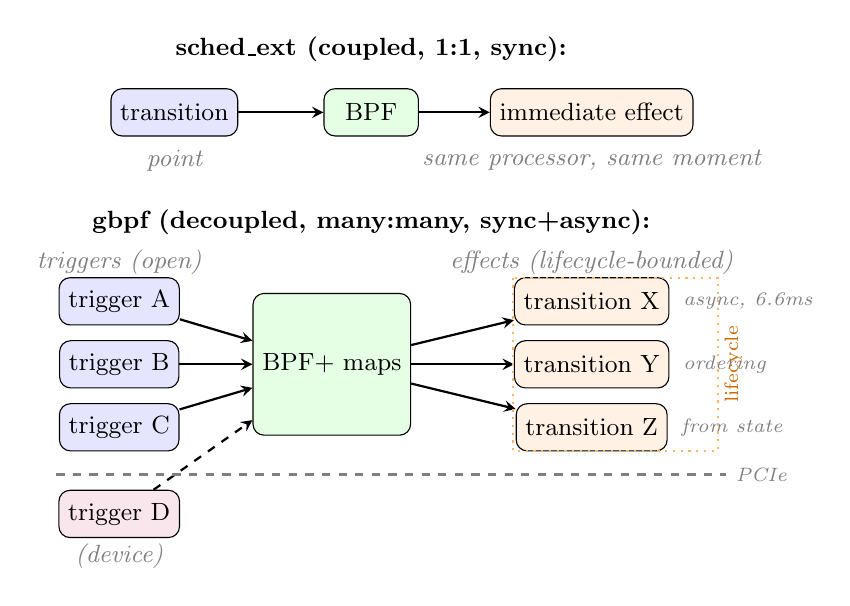
\begin{tikzpicture}[
  node distance=0.4cm and 0.6cm,
  box/.style={draw, rounded corners, minimum height=0.6cm, minimum width=1.2cm, font=\small},
  trigger/.style={box, fill=blue!10},
  bpf/.style={box, fill=green!10},
  effect/.style={box, fill=orange!10},
  label/.style={font=\small\itshape, text=gray},
  arrow/.style={->, >=stealth, thick},
  dasharrow/.style={->, >=stealth, thick, dashed},
  every node/.style={font=\small},
]

% === sched_ext (top half) ===
\node[font=\small\bfseries] (sched_title) at (0, 0) {sched\_ext (coupled, 1:1, sync):};

\node[trigger] (s_trans) at (-2.5, -0.8) {transition};
\node[bpf]     (s_bpf)   at (0, -0.8)    {BPF};
\node[effect]  (s_eff)   at (2.8, -0.8)   {immediate effect};

\draw[arrow] (s_trans) -- (s_bpf);
\draw[arrow] (s_bpf)   -- (s_eff);

\node[label, below=0.05cm of s_trans] {point};
\node[label, below=0.05cm of s_eff] {same processor, same moment};

% === gpu_ext (bottom half) ===
\node[font=\small\bfseries] (gpu_title) at (0, -2.2) {\sys{} (decoupled, many:many, sync+async):};

% Triggers
\node[trigger] (t_a) at (-3.2, -3.2) {trigger A};
\node[trigger] (t_b) at (-3.2, -4.0) {trigger B};
\node[trigger] (t_c) at (-3.2, -4.8) {trigger C};
\node[trigger, fill=purple!10] (t_d) at (-3.2, -5.9) {trigger D};
\node[label, below=-0.05cm of t_d] {(device)};

% BPF + maps
\node[bpf, minimum height=1.8cm, minimum width=1.4cm] (g_bpf) at (-0.5, -4.0) {BPF\\+ maps};

% Effects (lifecycle transitions)
\node[effect] (e_x) at (2.8, -3.2) {transition X};
\node[label, right=0.05cm of e_x] {\scriptsize async, 6.6ms};
\node[effect] (e_y) at (2.8, -4.0) {transition Y};
\node[label, right=0.05cm of e_y] {\scriptsize ordering};
\node[effect] (e_z) at (2.8, -4.8) {transition Z};
\node[label, right=0.05cm of e_z] {\scriptsize from state};

% Arrows from triggers to BPF
\draw[arrow] (t_a) -- (g_bpf);
\draw[arrow] (t_b) -- (g_bpf);
\draw[arrow] (t_c) -- (g_bpf);
\draw[dasharrow] (t_d) -- (g_bpf);

% Arrows from BPF to effects
\draw[arrow] (g_bpf) -- (e_x);
\draw[arrow] (g_bpf) -- (e_y);
\draw[arrow] (g_bpf) -- (e_z);

% PCIe boundary
\draw[thick, dashed, gray] (-4.0, -5.4) -- (4.5, -5.4) node[right, font=\scriptsize\itshape, text=gray] {PCIe};

% Labels
\node[label] at (-3.2, -2.7) {triggers (open)};
\node[label] at (2.8, -2.7) {effects (lifecycle-bounded)};

% Lifecycle boundary box
\draw[thick, dotted, orange!60] (1.8, -2.9) rectangle (4.4, -5.1);
\node[font=\scriptsize, orange!80!black, rotate=90] at (4.6, -4.0) {lifecycle};

\end{tikzpicture}
\caption{Execution model contrast. In sched\_ext, each BPF callback makes one synchronous decision at one transition point (coupled, 1:1). In \sys{}, BPF programs triggered from any point in the GPU management stack can direct multiple lifecycle transitions asynchronously via kfunc effects (decoupled, many:many). Triggers are open; effects are lifecycle-bounded. The dashed line marks the host-device boundary.}
\label{fig:exec-model}
\end{figure}



More broadly, device-side BPF enables three distinct usage patterns beyond host-only extensibility: (1)~\emph{observation feedback}, where device handlers write warp-level statistics to cross-layer maps that host policies read (the expert frequency example above); (2)~\emph{combined host-device policy}, where device-side and host-side programs cooperate on the same transition (e.g., device L2 prefetch triggers host callback for extended prefetch); and (3)~\emph{device-local policy}, where device-side BPF makes scheduling decisions entirely on-device (e.g., work-stealing block scheduler via \texttt{should\_try\_steal}). The SIMT-aware verifier and cross-layer maps exist precisely to enable all three patterns.



\subsubsection{Example: MoE Expert Offloading}

We illustrate the model with MoE expert offloading, a scenario that naturally requires all three layers. Consider a 120B Mixture-of-Experts model (59\,GiB) on a 32\,GB GPU: not all expert weights fit in device memory, so the driver must continuously evict and migrate pages. Each token activates only a subset of experts, but the default driver uses LRU eviction and tree-based prefetching, which are unaware of expert activation patterns. The result: every token triggers page faults on cold expert pages, each incurring milliseconds of PCIe DMA stall.

A \sys policy addresses this with three cooperating BPF programs across three layers, connected by a shared map. First, during inference, a device-side BPF handler monitors which expert pages each warp actually accesses, writing per-expert access counts to a cross-layer map; this information is invisible to the host, as only device-side BPF can observe warp-level access patterns within GPU kernel execution. Second, a BPF program attached to \texttt{cudaLaunchKernel} fires before each layer executes; it reads the device-side access map to predict which experts the next layer will activate, then calls \texttt{bpf\_gpu\_prefetch\_async} to migrate their pages before compute begins, avoiding the 6.6\,ms fault-driven DMA stall by overlapping migration with computation. In multi-tenant settings, the same program can simultaneously preempt a low-priority tenant's GPU context via \texttt{gdrv\_sched\_preempt} to free device memory for the prefetch, illustrating how memory and scheduling are coupled: prefetch requires free memory, which requires a scheduling decision. Third, when memory pressure requires eviction, the driver invokes a BPF handler at the \emph{evict\_prepare} lifecycle event; the handler reads the same access-frequency map and applies LFU ordering, protecting frequently-activated expert pages and evicting cold ones first. The kernel enforces safety, including fallback FIFO eviction under pressure.

\begin{lstlisting}
// Device-side: observe expert access patterns
SEC("gpu_dev/mem_access")
int moe_observe(gdev_mem_access_ctx_t *ctx) {
  u64 va = ctx->va & EXPERT_MASK;
  u64 *freq = bpf_map_lookup_elem(&expert_freq, &va);
  if (freq) __sync_fetch_and_add(freq, 1);
  return 0;
}

// Uprobe: prefetch + preempt at kernel launch
SEC("uprobe/cudaLaunchKernel")
int moe_prefetch(struct pt_regs *ctx) {
  u64 next_va = predict_next_expert(ctx);
  // Memory: prefetch predicted hot experts
  bpf_gpu_prefetch_async(next_va, EXPERT_SIZE);
  // Scheduling: preempt BE tenant to free memory
  if (bpf_gpu_mem_pressure() > THRESHOLD)
    gdrv_sched_preempt(BE_CONTEXT);
  return 0;
}

// Driver hook: evict cold experts, protect hot ones
SEC("gpu_mem/evict_prepare")
int moe_evict(gdrv_mem_remove_ctx_t *ctx) {
  gmem_region_t *r = ctx->region;
  u64 *freq = bpf_map_lookup_elem(&expert_freq,
                                   &r->va);
  if (freq && *freq > HOT_THRESHOLD)
    bpf_gpu_move_tail(&ctx->evict_list, r); // keep
  else
    bpf_gpu_move_head(&ctx->evict_list, r); // evict
  return 0;
}
\end{lstlisting}

Each layer exists because information resides in a different place: expert activation patterns are visible only on the device, application-layer intent is visible only at API calls, and eviction and scheduling decisions are made inside the driver. The three BPF programs coordinate through cross-layer maps, directing lifecycle transitions across both memory and scheduling domains from triggers that span the entire stack.

\subsubsection{Policy Safety and Correctness Guarantees}



The policy capability surface equals the kfunc set: policies can only invoke approved lifecycle operations. This guarantees correctness (no invalid transitions, no memory corruption) but not performance isolation; a policy can flood async prefetches or starve eviction, degrading throughput, just as a sched\_ext policy can dispatch to the wrong CPU. The remedy is the same: unload and fallback. Regardless of where a BPF program is triggered, it can only direct valid lifecycle transitions through kfuncs; each kfunc validates its parameters and enforces lifecycle invariants before executing. The BPF verifier guarantees that programs terminate and stay within memory bounds. If a policy errs or is unloaded, the driver reverts to default behavior.

\subsection{High-Level Architecture}
\label{sec:arch}

\begin{figure}
\centering
    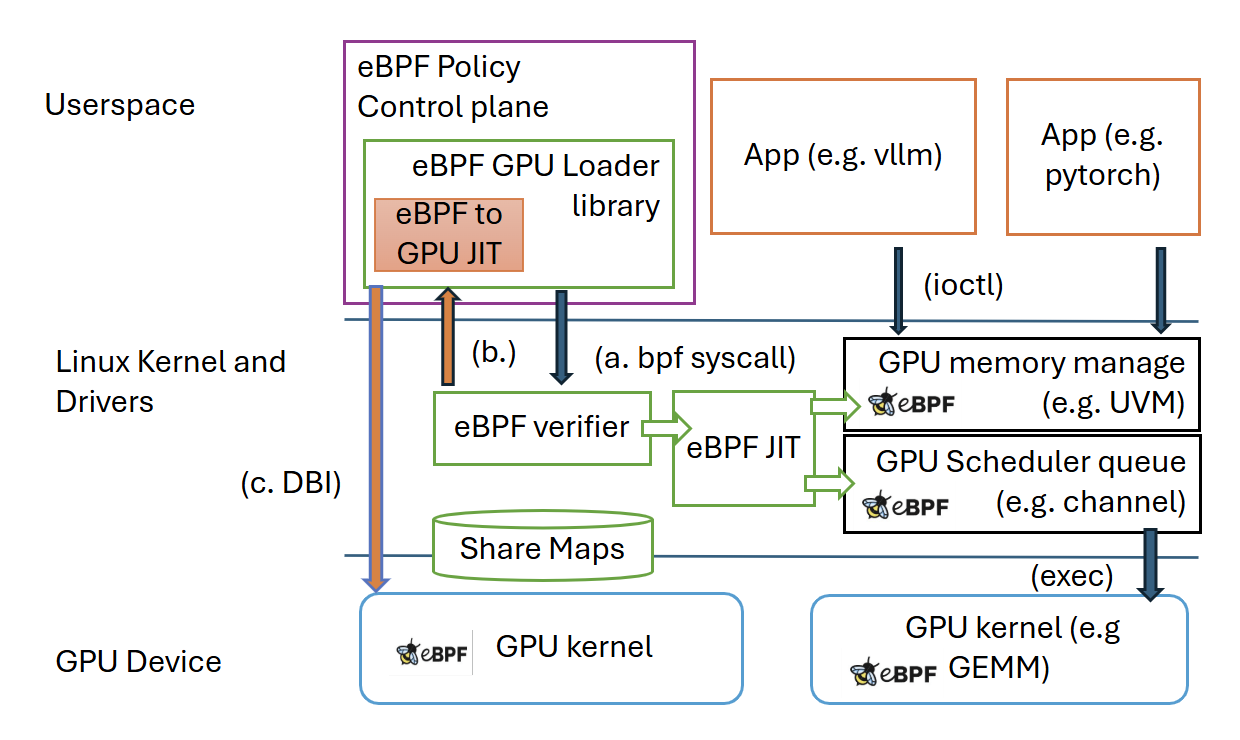
\includegraphics[width=\columnwidth]{img/gpu-ebpf-arch.png}
\vspace{-.5ex}
\caption{\sys architecture: cross-layer eBPF runtime spanning kernel driver and GPU device. The control plane deploys policies via (a) bpf syscall to verifier and driver hooks (b) GPU JIT after verification; (c) DBI injects trampolines into GPU kernels. Shared maps enable state coordination across layers.}
\label{fig:system-design}
\end{figure}

Figure~\ref{fig:system-design} shows how \sys realizes this execution model.

\paragraph{User-space Control Plane.}
Policy authors use standard eBPF tooling (e.g., \texttt{clang/libbpf}, \texttt{bpftool}) to build policy bytecode. The control-plane links against a loader library that installs policies and configures eBPF maps. It enables runtime policy redeployment and reconfiguration (e.g., eviction thresholds, sampling rates, priorities) without application or kernel restarts, and exports runtime metrics (e.g., region hotness, tenant latencies).

\paragraph{Host Driver and Device Runtime.}
\sys provides a unified runtime across host driver and GPU device contexts, managing verification, compilation, and map placement. It employs a SIMT-aware verifier (\S\ref{sec:verification}) that extends standard eBPF checks to verify warp-uniformity, SIMT control flow, and GPU synchronization constraints. Verified programs are JIT-compiled into native host code or GPU-compatible instructions (e.g., PTX). The runtime manages hierarchical logical eBPF map abstractions whose backing storage is automatically partitioned and replicated across host and device with consistency.
Policy execution occurs at structured hook points defined in GPU drivers and device. On the host, \sysdriver exposes \texttt{struct\_ops}-style hooks (e.g., region activate/eviction, GPU kernel scheduling). Host policies return concise policy decisions enforced via trusted kfuncs. On the GPU device, \sys injects trampolines at hook points and invokes device-side handlers at warp granularity. Device handlers update cross-layer maps with performance signals and make control decisions (e.g., prefetch, block-level scheduling) via trusted helpers that the runtime enforces.

\subsection{Runtime Verification and Optimizations}
\label{sec:verification}

\sys policies execute directly within privileged GPU driver and kernel contexts, making safety guarantees critical. We adopt a standard eBPF threat model: we trust system administrators loading policies, but consider policy code potentially buggy or misconfigured. The trusted computing base (TCB) includes the kernel and \sys kernel module, GPU compiler backend, and GPU driver/firmware. Policy authors only interact with eBPF and do not write native device code. For host-side verification, we reuse the existing Linux kernel eBPF verifier unchanged, relying on standard type-checking, bounded-loop, and memory-safety constraints. \sys-specific kfuncs and hooks are declared via BPF Type Format (BTF) metadata.

\subsubsection{SIMT-aware Verification}

Because the GPU executes in SIMT (Single Instruction, Multiple Threads) mode, device-side BPF programs must respect warp-level execution semantics. \sys introduces a SIMT-aware static verification model enforcing warp-level uniformity constraints to ensure efficient and safe GPU-side policy execution.
The key insight is that we distinguish \emph{warp-uniform} values (identical across warp threads, e.g., region identifiers) from \emph{lane-varying} values (thread-local GPU state). Policies may compute freely using lane-varying values, but these must not influence control-flow decisions or directly produce side effects visible outside a warp. To guarantee warp-level coherence, \sys mandates that branch conditions, loop bounds, and map-update keys be warp-uniform or derived via warp-level aggregation. Additionally, \sys prohibits GPU-wide barriers, global synchronization primitives, and non-uniform atomic operations, and imposes resource budgets per policy hook to bound memory and thread resource usage. These constraints ensure safe policy integration that respects GPU hardware execution semantics.

\subsubsection{Warp-level Execution Optimizations}

Direct scalar execution of eBPF after SIMT verification on GPU threads still causes resource overhead (e.g. duplicate memory update to maps) due to the SIMT. To resolve this, \sys introduces a warp-level aggregated execution model, executing policy logic once per warp using a designated "warp leader" (typically lane 0). Each hook invocation conceptually follows a two-phase approach: each lane independently computes lane-local contributions (e.g., effective addresses, counters) without influencing control flow or directly updating shared state. These contributions are then aggregated at warp granularity. Subsequently, the warp leader executes the policy handler once using aggregated inputs and warp-uniform context. The resulting decision is broadcast back to all lanes. This design minimizes GPU overhead while preserving eBPF's scalar semantics. To further reduce runtime overhead, \sys employs compiler-level optimizations (specialization and inlining) tailored for warp-level execution.

\subsubsection{Hierarchical Cross-layer Maps for State Coordination}

GPU policy decisions require coherent sharing of policy state across asynchronous CPU and GPU contexts. To transparently bridge CPU-GPU memory hierarchies, \sys introduces cross-layer maps. Logically, each map is a single unified key-value store accessible from host-side driver hooks, GPU-side device policies, and user-space control planes, and verifiable through eBPF's existing model. Physically, maps are realized as hierarchical shards across host DRAM, GPU global memory, and GPU-local storage (e.g., shared memory, SM-local). The runtime dynamically determines shard placement based on access frequency, latency, and capacity constraints. Following eBPF's soft-state philosophy, \sys maps provide relaxed, eventual consistency. Instead of strong global ordering, our runtime periodically merges GPU-local map shards into canonical snapshots at synchronization points, such as GPU kernel completion boundaries. This snapshot-based model is sufficient for policy decisions relying on approximate statistics. Occasional staleness affects decision optimality but cannot violate correctness invariants such as memory integrity, which remain enforced by the GPU driver and hardware MMU.


\section{Implementation}
\label{sec:implementation}

\subsection{Components Overview}

We implemented \sys on Linux 6.15, extending the kernel with a standalone file ($\sim$1 KLOC) that handles hook registration and verifier extensions. Additionally, we integrated lightweight instrumentation ($\sim$100 LOC) into NVIDIA's open GPU kernel modules to expose key memory management and scheduling decision points (\S\ref{sec:impl-host}). Our userspace loader and JIT infrastructure ($\sim$10 KLOC) builds upon bpftime's framework, while an LLVM-based backend ($\sim$1 KLOC) translates the restricted \sys eBPF instruction subset into GPU device code (PTX/SPIR-V).

\subsection{Host-side Integration}
\label{sec:impl-host}

\sys extends the NVIDIA Open GPU Kernel Modules (Turing, Ampere, Hopper, Blackwell, and newer), specifically instrumenting the UVM module at critical memory-management decision points such as the page fault handler and prefetch logic. At each hook, the driver constructs a compact context containing relevant fields (e.g., region range, fault address, block size) and invokes an attached eBPF handler. Each handler returns a small enumerated decision indicating whether to execute the default kernel logic or bypass it with custom behavior. We instrument the lifecycle events of GPU hardware queues, each corresponding to a Time-Slice Group (TSG). Specifically, we add hooks at TSG initialization (\texttt{queue_create}) and teardown (\texttt{queue_destroy}). The eBPF handlers attached to these hooks configure scheduling parameters such as TSG priority, timeslice duration, and runlist interleave frequency. Additionally, policies can cooperatively preempt active TSGs via the \texttt{gdrv_sched_preempt} kfunc, invoking the driver's existing context-switch mechanism. Our kernel module directly extends the standard Linux eBPF verifier by registering GPU-specific attach points and kfunc interfaces. The verifier extension leverages BTF annotations and kfunc type signatures to rigorously enforce type and memory safety, safely exposing critical driver-level actions such as eviction candidate selection and kernel preemption to verified eBPF handlers.


\subsection{GPU Runtime}
\label{sec:impl-gpu}

\paragraph{Code Generation and Binary Trampolines.}

Once a \sys eBPF program passes verification and is loaded into the kernel, our loader intercepts its bytecode and BTF metadata, then forwards them to our userspace backend for GPU code generation (PTX/SPIR-V). Verified code executes either directly in the kernel (using the standard eBPF JIT) or on the GPU through our specialized backend and runtime. To support runtime instrumentation without recompilation overhead, \sys dynamically injects lightweight binary trampolines at strategic kernel points (entry points, selected memory instructions, and execution-phase boundaries). We also expose a minimal set of runtime helper functions, pre-compiled to GPU device code with verifier-approved signatures. During translation, static analysis ensures minimal context structures are constructed, only materializing fields referenced by handlers, and inserts prologue/epilogue logic to manage SIMT-aware register state preservation. By directly translating verified eBPF bytecode to GPU-executable code, \sys seamlessly extends Linux's kernel-level safety guarantees (e.g. memory safety, bounded loops, and type safety) into GPU kernels.

\paragraph{Scheduling and Memory Operations.}

For scheduling policies, \sys employs a thread-block scheduler abstraction that models kernel execution as dynamically scheduled units of work (e.g., tiles or logical blocks), executed by persistent worker blocks. On Blackwell GPUs, we leverage hardware-supported cluster launch control APIs, which treat block grids as dynamically manageable tasks, enabling efficient hardware-supported work-stealing. Each GPU worker executes its assigned unit, invokes device-side \sys policy handlers (running in dedicated SIMT lanes) to select or approve subsequent tasks, and interacts with the cluster control APIs to claim or relinquish tasks. Execution-phase annotations and instrumentation points are implemented via low-overhead \sys trampolines. Critically, all GPU-resident scheduling logic strictly adheres to bounded-execution constraints enforced by our verifier.

For memory management, \sys attaches handlers to select memory instructions, device-side tracepoints, or kernel function boundaries, allowing policies to issue lightweight hints back to the host driver through helper calls. In contrast to prior GPU instrumentation efforts (e.g., eGPU) that rely on expensive atomic synchronization and fences, \sys helper functions and instrumentation logic avoid explicit synchronization primitives, significantly minimizing overhead.

\paragraph{Cross-Domain State and Synchronization.}

\sys relies on standard eBPF maps as its unified state abstraction across host-driver and GPU-device boundaries. To ensure efficient, zero-copy synchronization, we allocate map structures within GPU-accessible unified memory regions, thereby eliminating explicit data marshalling overhead between CPU and GPU contexts. These shared maps maintain dynamic policy state such as per-region access frequency (hotness), per-tenant scheduling priorities, block-level execution progress, and instrumentation counters. Unlike previous eGPU implementations, which restricted maps exclusively to CPU memory, causing prohibitive synchronization overhead, \sys transparently supports placing frequently accessed policy state directly within GPU registers, GPU local memory, or CPU-side memory, enabling optimal locality and minimal runtime overhead.

\subsection{SIMT-aware Verification Implementation}
\label{sec:impl-verification}

The host-side verifier uses Linux kernel's existing eBPF verifier without modification, ensuring standard memory safety, bounded loops, and resource usage. We implement our GPU-specific extensions by adding an extra verification pass at program load time within the kernel module. This pass statically identifies warp-uniform fields from context structures annotated via BTF metadata. The verifier then performs conservative dataflow analysis: each register and stack slot is tagged as uniform or varying, and these tags propagate through arithmetic and logical operations. Combining two uniform values yields uniform; any operation involving a varying operand yields varying; helper return values use uniformity annotations from their BTF declarations. Control flow analysis checks that branches and loops depend solely on these warp-uniform fields, explicitly rejecting programs violating this constraint. Map update operations are additionally checked to ensure keys are warp-uniform.

We enforce resource bounds per hook type, setting conservative instruction and memory-operation budgets based on the expected trigger frequency and latency budget of each hook. Our verifier explicitly rejects GPU-wide synchronization constructs, global barriers, and non-uniform atomic operations that could cause hardware stalls or memory consistency violations. No runtime sandboxing mechanisms are used; policies that pass verification run directly on GPU hardware, while rejected programs are never executed.

\subsection{Warp-level Execution Implementation}

The GPU runtime implements warp-level execution aggregation via lightweight device-side trampolines inserted at kernel entry, synchronization barriers, and critical memory instructions. The two-phase execution model is realized as follows: in the lane-local phase, each lane computes its per-thread contributions (e.g., effective addresses, partial counters) into registers; these are then aggregated using \texttt{\_\_ballot\_sync} for masks and \texttt{\_\_shfl\_sync} for value reduction. In the warp-policy phase, lane~0 (or the first active lane via \texttt{\_\_ffs(\_\_activemask())}) executes the translated eBPF handler with the aggregated inputs. Trampolines minimally save warp execution state, aggregate lane-varying inputs using GPU shuffle instructions, execute the scalar policy handler once per warp, and then broadcast results back to all threads using shuffle operations.

We implement aggressive function and map-helper call inlining at JIT compilation, significantly reducing call overhead and branching. GPU map operations are specialized by identifying common access patterns and embedding them directly into the handler code, reducing register pressure and avoiding global memory round trips. An optional sampling mechanism is also provided to allow dynamic control of policy overhead.

\subsection{Hierarchical Map Implementation}

Our runtime internally employs a cost-based heuristic placement model for cross-layer maps. Low-frequency global state is stored in CPU host DRAM with periodic GPU-side snapshots cached locally. Frequently accessed GPU-intensive state is primarily stored in GPU global memory, periodically aggregated and asynchronously flushed back to host memory for policy consumption. Extremely hot per-warp or per-SM data resides directly in GPU shared memory or SM-local storage, ensuring extremely low latency access.

Device-side handlers use standard eBPF helper APIs to access maps, fully unaware of underlying memory management complexity. Per-key atomicity is implemented using native GPU atomic operations for single-key updates. The snapshot-based consistency model is realized by defining merge points at GPU kernel completion boundaries: when a kernel finishes, the runtime triggers an asynchronous flush of GPU-local map shards to canonical instances in global memory or host DRAM. Host-side handlers and user-space control-plane logic observe these coherent snapshots rather than in-flight GPU-side updates.

As a concrete example, GPU-side memory-access instrumentation handlers record per-region statistics directly into GPU-local map shards. Periodically, the runtime aggregates these shards into global GPU memory, subsequently making them available to host-side handlers. Host-side eviction handlers then read coherent aggregate statistics directly from global maps, enabling accurate memory management decisions without explicit data movement or synchronization logic in policy handlers.

\section{Use Case}

\subsection{GPU Memory Tracer}\label{sec:use_case_gpu_memory_tracer}
\noindent \sys instruments LD/ST sites via PTX trampolines and logs address, size, warp/SM IDs, and timestamps into a shared eBPF map. A user-space consumer derives bandwidth, coalescing, and contention metrics with sub-\(\mu\)s latency, enabling quick diagnosis of bank conflicts or uncoalesced accesses without relaunching kernels.

\subsection{Fair Share Scheduling}\label{sec:use_case_fair_share}
\noindent Block-level entry/exit probes report per-block runtimes into shared maps. A host scheduler adjusts future block quotas to equalize progress across tenants, yielding near-ideal Jain's fairness with \(<2\%\) overhead while remaining transparent to application code and CUDA streams.

\subsection{ML Green: CPU–GPU Collaborative Inference}
\noindent For models that exceed on-device memory or under renewable-aware power budgets, \sys traces tensor access patterns to guide split execution akin to Neuro-Surgeon~\cite{neurosurgeon}. Policies such as LRU/LFU and full-CPU/full-GPU offload are evaluated online; access and energy traces steer eviction and prefetch so transfers overlap compute under varying power availability.


\section{Evaluation}
\label{sec:eval}

We evaluate \sys along five questions:

\begin{itemize}[leftmargin=*]
  \item \textbf{RQ1:} What is the runtime overhead of the \sys runtime compared
        to existing GPU instrumentation frameworks?
  \item \textbf{RQ2:} How efficiently can \sys maintain shared state across the
        CPU–GPU boundary?
  \item \textbf{RQ3:} Can \sys express practical GPU observability tools with
        significantly lower overhead than CUPTI and NVBit?
  \item \textbf{RQ4:} Can \sys-based memory policies improve performance over
        default UVM behavior across different access patterns?
  \item \textbf{RQ5:} Can \sys-based scheduling policies provide tangible gains
        in tail latency, throughput, and power efficiency in mixed workloads?
\end{itemize}

\subsection{Methodology and Setup}

We evaluated \sys on two machines. Server~A is a single-socket Intel Core Ultra~9
285K processor (24 cores) with 128~GB DDR5 RAM and an NVIDIA RTX~5090 GPU.
Server~B is a single-socket Intel Xeon~6787P (86~cores, 2.0~GHz, 336~MB LLC)
with 768~GB DDR5 RAM (512~GB CXL module) and an NVIDIA H100 GPU. Unless
otherwise noted, we report results on Server~A and average each metric over
10 trials; when averaging speedups we use geometric means. We compare against
NVIDIA's CUPTI and NVTX-based profiler stack, NVBit gpumemtrace, default UVM
memory management, and the native GPU scheduler without \sys-based policies.

\subsection{RQ1: Runtime Overhead vs Existing Tools}

We first quantify the overhead of the \sys runtime itself, independent of any
specific policy logic. We use two microbenchmarks:

\begin{itemize}[leftmargin=*]
  \item A load/store latency benchmark that issues controlled memory accesses
        from GPU kernels, instrumented with \sys and with NVBit gpumemtrace.
  \item A ResNet inference workload instrumented with \sys-based tracing and
        with the PyTorch profiler (CUPTI+NVTX).
\end{itemize}

\Cref{fig:runtime-overhead} shows the per-access latency slowdown under
\sys and NVBit as access sizes increase. \sys adds substantially less latency
than NVBit, remaining low and stable below 128~KB and increasing modestly
thereafter. \Cref{fig:resnet-latency} compares end-to-end ResNet inference
latency distributions: p10 and mean latencies are slightly better than under the PyTorch profiler, and p99 latency is comparable. In both
cases, lightweight launch-time injection and warp-level execution of \sys
handlers are key to keeping overhead low.

\begin{figure} \centering \fbox{\parbox{0.5\textwidth}{\centering [Figure: Runtime Overhead]}} \caption{Runtime Overhead} \label{fig:runtime-overhead} \end{figure}

\begin{figure} \centering \fbox{\parbox{0.5\textwidth}{\centering [Figure: Resnet Inference Latency Overhead]}} \caption{Resnet Inference Latency Overhead} \label{fig:resnet-latency} \end{figure}

\subsection{RQ2: Shared State and Cross-domain Overheads}

Next, we measure the cost of maintaining shared state between CPU and GPU via
\sys maps. We benchmark shared-memory bandwidth and one-way latency on both
servers using a 1~GiB region and both GPU-to-CPU and CPU-to-GPU access patterns.
Servers~A and~B deliver 12–18~GB/s over PCIe with 8–15~µs cross-domain latencies,
which is sufficient for the policy state sizes we maintain. Our SIMT-aware
aggregation and sampling strategies further reduce the frequency of cross-domain
synchronization, as we validate in the use cases below.

\subsection{RQ3: Low-overhead GPU Observability}

We evaluate the suite of bcc-style observability tools built on \sys, measuring
accuracy, overhead, and practical utility across diverse workloads.

\paragraph{Thread divergence and workload balance.}
\texttt{kernelretsnoop} attaches to kernel return paths and records per-thread
timestamps, revealing divergence. Applied to a matrix multiply kernel with
boundary checks, it shows that threads handling edge cases (5% of total) incur
600–850~ns longer execution than interior threads, with timestamps within 10~ns
of hardware performance counters and 2.1% overhead. Refactoring boundary
handling based on this insight improves overall kernel performance by 8%.
\texttt{threadhist} reveals load imbalance in a particle simulation, identifying
a bimodal distribution of iterations per thread that, when corrected, yields an
18% throughput improvement with 1.8% tool overhead.

\paragraph{Launch latency and memory behavior.}
\texttt{launchlate} combines host and device hooks to measure kernel launch
latency. On a pipeline of 50 small kernels, default synchronous execution shows
150–550~µs launch latency per kernel, leading to 32~ms total runtime; switching
to CUDA graphs guided by \texttt{launchlate} reduces this to 7.2~ms. The tool
adds less than 0.5% overhead. \texttt{mem_trace} instruments sampled memory
operations and recovers per-warp bank conflict rates within 2% of hardware
counters, with under 3% end-to-end overhead across GEMM, SpMV, and stencil
kernels (\Cref{fig:obs-overhead}).

\begin{figure}
\centering
\fbox{\parbox{\columnwidth}{\centering [Figure: GPU Observability Tools Overhead Comparison]}}
\caption{Overhead comparison for bcc-style GPU observability tools across different workloads}\label{fig:obs-overhead}
\end{figure}


\paragraph{Comparison to CUPTI and NVBit.}
\Cref{fig:obs-comparison} compares \sys-based tools against CUPTI and
NVBit for common profiling tasks. CUPTI-based profiling incurs 15–25% overhead
and typically requires kernel restarts; NVBit adds 30–45% overhead for similar
metrics. \sys tools average 2–3% overhead and support live instrumentation
without interrupting execution.

\begin{figure}
\centering
\fbox{\parbox{\columnwidth}{\centering [Figure: Observability Tool Comparison]}}
\caption{Comparison of \sys observability tools vs. CUPTI and NVBit for common profiling tasks}\label{fig:obs-comparison}
\end{figure}


\subsection{RQ4: Programmable Memory Management}

We evaluate \sys's memory policy interface on workloads with diverse access
patterns: sequential (vector addition), strided (matrix transpose), and random
(graph traversal). We compare three configurations: (1) default NVIDIA UVM with
on-demand page migration, (2) static prefetching with manual hints, and (3) \sys
with adaptive region-based prefetch and eviction policies that use both host-side
events and device-side memory events.

\Cref{fig:uvm-perf} shows normalized execution time across workloads.
For sequential access, \sys achieves up to 1.8$\times$ speedup over default UVM
by prefetching consecutive regions based on observed access and device hints.
For strided patterns, \sys learns strides and prefetches accordingly, achieving
1.4$\times$ speedup. Random access sees a modest 1.2$\times$ improvement from
working-set tracking and retention of hot regions.

\Cref{fig:page-faults} shows page fault rates. Default UVM incurs 15–30K
faults per second depending on the workload; \sys reduces this to 5–12K~faults/s
(50–65% reduction) through predictive prefetching and more selective eviction.
The adaptive policy adds only 2–3% instrumentation overhead while eliminating
the majority of fault-induced stalls. Average memory footprint increases by
10–15%, which we bound using a hybrid policy that throttles prefetch aggressiveness
under tight capacity constraints, keeping performance within 5% of an
unbounded-memory configuration.

\begin{figure}
\centering
\fbox{\parbox{\columnwidth}{\centering [Figure: UVM Performance Comparison]}}
\caption{Normalized execution time for UVM management strategies across different access patterns}\label{fig:uvm-perf}
\end{figure}

\begin{figure}
\centering
\fbox{\parbox{\columnwidth}{\centering [Figure: Page Fault Frequency]}}
\caption{Page fault frequency comparison between default UVM and \sys programmable UVM}\label{fig:page-faults}
\end{figure}

\subsection{RQ5: Fine-grain Scheduling and Power-aware Control}

Finally, we evaluate \sys's scheduling interface using two classes of policies:
priority-based preemption and power-aware throttling, on mixed workloads that
combine high-priority latency-sensitive kernels (real-time video processing)
with low-priority batch ML training jobs.

\paragraph{Priority-based preemption.}
We compare three approaches: (1) no prioritization (FIFO), (2) CUDA stream-level
priorities, and (3) \sys-based warp-level preemption. \Cref{fig:p99-latency}
plots p99 latency for high-priority tasks. FIFO exhibits 25–80~ms p99 latency
due to blocking behind long-running kernels. CUDA streams reduce p99 to 15–30~ms
but still suffer head-of-line blocking. \sys cuts p99 latency to 5–12~ms by
preempting low-priority warps at synchronization points and handing resources
to high-priority work, with 4–6% overhead and 0.3–0.8~µs per scheduling decision.
Low-priority throughput drops by 8–12%, but \sys maintains better fairness than
CUDA streams, which incur 18–25% throughput reduction due to prolonged starvation
(\Cref{fig:lowprio-throughput}).

\begin{figure}
\centering
\fbox{\parbox{\columnwidth}{\centering [Figure: Priority Scheduler Tail Latency]}}
\caption{P99 latency for high-priority tasks under different scheduling policies}\label{fig:p99-latency}
\end{figure}

\begin{figure}
\centering
\fbox{\parbox{\columnwidth}{\centering [Figure: Low-Priority Task Throughput]}}
\caption{Throughput impact on low-priority tasks with different scheduling policies}\label{fig:lowprio-throughput}
\end{figure}

\paragraph{Power-aware throttling.}
We implement a thermal-aware scheduler that throttles thread blocks when GPU
temperature exceeds configured thresholds. \Cref{fig:power-throttle} shows
power consumption and performance over time under sustained load. Without
throttling, power spikes to 320~W and violates thermal limits. NVIDIA's frequency
scaling reduces power to 280~W but lowers performance by 20%. \sys's selective
thread throttling maintains 290~W average power while reducing performance by
only 8%, improving performance-per-watt compared to frequency scaling. The
sub-microsecond decision latency of \sys policies allows them to react to thermal
events before hardware protection mechanisms trigger.

\begin{figure}
\centering
\fbox{\parbox{\columnwidth}{\centering [Figure: Power-aware Throttling]}}
\caption{Power consumption and performance under thermal-aware throttling policies}\label{fig:power-throttle}
\end{figure}
\section{Related Work}\label{sec:related_work}
\xiangyu{simplify the description of each part in the related work because they are far from the focus of this paper.}
\subsection{Pure PTX injection for GPU Telemetry}
The Neutrino framework\cite{neutrino} pioneers zero-instrumentation GPU monitoring by leveraging PTX injection and hooks on CUDA runtime libraries. Without modifying application code, Neutrino attaches to user-level CUDA APIs to extract memory‐allocation patterns, kernel launch events, and resource‐usage metrics. It maps these events into isolated memory and delivers them to user space for visualization or offline analysis. This approach demonstrates that fine-grained GPU observability can be achieved with minimal overhead, and it provides a foundation upon which more advanced dynamic instrumentation and programmable tracing techniques can be built. However, it does not have the dynamism, CPU-GPU collaboration, and safety requirements that \sys provides.
   
\subsection{AI Observability Infrastructure}
Meta’s multi-layered observability stack\cite{ai-observability} combines low-overhead telemetry (via Dynolog and DCGM) with selective tracing (via CUPTI) to collect fleet-wide GPU metrics. Profiling tools such as PyTorch Profiler, Kineto, and Strobelight/BPF enable secure, real-time introspection of CUDA and PyTorch operations. An automated Analysis Platform stitches traces across hosts and highlights common inefficiencies—data starvation, kernel imbalances, or memory leaks—so developers can target optimizations effectively. Resource-attribution dashboards then allocate GPU hours or FLOPs by model or team, guiding long-term tuning efforts. Large-scale data centers require automated telemetry collection and analysis. Google’s GPU sharing on Kubernetes highlights orchestration at scale, while Meta’s Performance Profiling Platform automates trace stitching, anomaly detection, and trend analysis across thousands of jobs. These platforms underscore the necessity of coupling low-overhead data collection with intelligent, fleet-wide aggregation—an approach that informs \sys’s design for seamless integration into existing observability pipelines.

\subsection{Reducing Energy Usage in LLM training and inference}
Neurosurgeon\cite{neurosurgeon} introduces a framework for partitioning deep neural network inference between mobile devices and cloud servers to optimize end-to-end latency and energy consumption. By profiling layer-wise execution characteristics and network conditions, Neurosurgeon determines optimal split points in the model where computation should shift from edge to cloud. This collaborative intelligence approach enables resource-constrained devices to leverage cloud GPU power dynamically, reducing on-device latency and energy usage while maintaining accuracy. Perseus\cite{chung2024reducing} addresses the growing energy bottleneck in large-scale generative AI training by identifying and mitigating \emph{energy bloat}—energy consumed without contributing to throughput. It categorizes bloat into intrinsic (workload imbalance across pipeline parallel stages) and extrinsic (straggler-induced stalls in multi-pipeline training) sources. Perseus constructs the iteration time–energy Pareto frontier via an efficient graph–cut–based algorithm, then dynamically adjusts GPU frequency plans per computation to minimize total energy consumption without sacrificing throughput. Evaluations on models like GPT-3 demonstrate up to 30\% energy savings with negligible performance loss.

\section{Conclusion}
\label{sec:conclusion}
% Our comprehensive evaluation confirms that \sys{} not only meets but exceeds our initial expectations. 
\xiangyu{We build \sys{} that offloads eBPF bytecode to monitor GPU's runtime performance using dynamic PTX injection. On standard NVIDIA servers, \sys{} reduces instrumentation overhead, boosts throughput and cut the CPU-GPU round trip latency. 
These improvements translate directly into smoother, more balanced pipelines without frequent kernel launches. 
The results demonstrate that \sys{}’s shared-memory approach and flexible PTX injection scale seamlessly to Grace Hopper–class architectures, delivering a fully responsive, high-throughput observability and programmability framework for GPU-driven workloads.}

% On a standard NVIDIA P40 and H100 server, \sys{} reduces instrumentation overhead from 5.2\% (baseline uprobe tracing) to just 1.8\% on average, while boosting throughput for streaming workloads by 23\%. We cut CPU–GPU round-trip latency by 34\%, and dynamic PTX injection completes in under 20 µs—ensuring long-running kernels remain fully occupied even under irregular or fine-grained task patterns. These improvements translate directly into smoother, more balanced pipelines without frequent kernel launches.

% Crucially, we have now validated \sys{} on a production-scale NVIDIA Grace CPU + Hopper GPU node, another machine with a GPU interconnected via CXL memory pooling. The results demonstrate that \sys{}’s shared-memory approach and flexible PTX injection scale seamlessly to Grace Hopper–class architectures, delivering a fully responsive, high-throughput observability and programmability framework for today’s and tomorrow’s GPU-driven workloads.

% 参考文献：USENIX 模板通常用 plain 或 abbrvnat 等
\bibliographystyle{plain}
\bibliography{cite}

\end{document}
